\chapter{The Collatz Tree}

\section{The Connection between Groups and Graphs}
\label{sec:groups_graphs}
Let $(a_k)$ be a numerical sequence with $a_k=g^{(k)}(m)$, then a reversion produces an infinite number of sequences of reversely-written Collatz members \cite{Ref_Klisse_2010}.

\par\medskip
Let $S$ be a set containing two elements $q$ and $r$, which are bijective 
functions over $\mathbb{Q}$:
\begin{equation}
\begin{array}{l}
q(x)=2x \\ 
r(x)=\frac{1}{3}(x-1)
\end{array}
\end{equation}

Let a binary operation be the right-to-left composition of functions
$q\circ r$, where $q\circ r(x)=q(r(x))$. Composing functions is an
associative operation. All compositions of the bijections $q$ and $r$
and their inverses $q^{-1}$ and $r^{-1}$ are again bijective. The set,
whose elements are all these compositions, is closed under that operation.
It forms a free group $F$ of rank 2 with respect to the free generating set $S$, where the group's binary operation $\circ$ is the function composition and the group's identity element is the identity function $id_{\mathbb{Q}}=e$. We call $e$ an \textit{empty string}. $F$ consists of all expressions (strings) that can be concatenated from the generators $q$ and $r$. The corresponding Cayley graph $Cay(F,S)=G$ is a regular tree whose vertices have four neighbors \cite[p.~66]{Ref_Loeh}. A tree is called \textit{regular} or \textit{homogeneous} when every vertex has the same degree, in this case, $d(v)=4$ for every vertex $v$ in $G$. The Cayley graph's set of vertices is $V(G)=F$, and its set of edges is $E(G)=\left\{\left\{f,f\circ s\right\}\mid f\in F,s\in\left(S\cup S^{-1}\right)\setminus\left\{e\right\}\right\}$ \cite[p.~57]{Ref_Loeh}. More precisely, the vertices are \textit{labeled} by the elements (strings) of $F$.

\par\medskip
In conformance with graph-theoretical precepts \cite{Ref_Bondy_Murty},
\cite{Ref_Bonnington_Little}, \cite{Ref_Bender_Williamson}
we specify a subgraph $H$ of $G$ as a triple
$\left(V(H),E(H),\psi_{H}\right)$ consisting of a set $V(H)$ of vertices,
a set $E(H)$ of edges, and an incidence function $\psi_{H}$. The latter
is, in our case, the restriction $\psi_{G}\vert_{E(H)}$ of the Cayley
graph's incidence function to the set of edges that only join vertices,
which are labeled by a string over alphabet $\{r,q\}$ without the inverses:
$E(H)=\left\{\left\{f,f\circ s\right\}\mid f\in F,s\in S\setminus\left\{e
\right\}\right\}$.

\par\medskip
This subgraph corresponds to the monoid $S^*$, which is freely generated
by $S$ follows related thoughts \cite{Ref_Truemper_2014} that examine
the Collatz problem in terms of a free semigroup on the set $S^{-1}$ of
inverse generators. Note that this semigroup is not to be confused with an
\textit{inverse semigroup} "in which every element has a unique inverse"
\cite[p.~26]{Ref_Almeida}, \cite[p.~22]{Ref_Loeh}.

\par\medskip
Let $Y^X=\{f\mid f\text{ is a map }X\rightarrow Y\}$ be the set of functions, which in category theory is referred to as the \textit{exponential object} for any sets $X$, $Y$. The evaluation function $ev:Y^X\times X\to Y$ sends the pair $(f,x)$ to $f(x)$. For a detailed description of this concept, see \cite[p.~127]{Ref_Johnsonbaugh}, \cite[p.~155]{Ref_MacLane_Birkhoff}, \cite[p.~54]{Ref_Novak_etal} and \cite[p.~188]{Ref_Pellissier}. We define the evaluation function $ev_{S^*}:S^*\times\{1\}\rightarrow\mathbb{Q}$ that evaluates an element of $S^*$, id est a composition of $q$ and $r$, for the given input value $1$. Furthermore we define the corestriction ${ev^0_{S^*}}$ of $ev_{S^*}$ to $\mathbb{N}$. Since a corestricion of a function resricts the function's codomain \cite[p.~3]{Ref_Helemskii}, the function $ev^0_{S^*}$ operates on a subset $T\subset S^*$ that contains only those compositions of $q$ and $r$, which return a natural number when inputting the value $1$.

\par\medskip
The set $T$ forms not a monoid under function composition, for example $ev_{S^*}(qrq^4,1)=10$ and $ev_{S^*}(rq^6,1)=21$, but the composition $qrq^4rq^6$ does not lie in $T$, because the evaluation $ev_{S^*}(qrq^4rq^6,1)$ yields a value outside the codomain $\mathbb{N}$. However, each element of this set labels a vertex of a tree $H_{T}\subset H$, which is a proper subtree of $H$.

\par\medskip
Let $U\subset T$ be a subset of $T$, which does not contain a reduced word with two or more successive characters $r$. The corresponding tree $H_{U}\subset H_{T}$ reflects Collatz sequences as demonstrated in figure~\ref{fig:1}.

\par\bigskip
\begin{remark}
When talking about trees having a root ("rooted trees"), another important concept should be explained: the \textbf{level of a vertex} or often called \textbf{depth of a vertex} is the length of the path from the root to this vertex \cite[p.~804]{Ref_Rosen}. In other words, it is the vertex's distance (the number of edges in the path) from the root. The \textbf{height of a vertex} is its level plus one $level(v)+1=height(v)$, see \cite[p.~169]{Ref_Makinson}.
\end{remark}

% trim=left top right bottom
\begin{figure}
	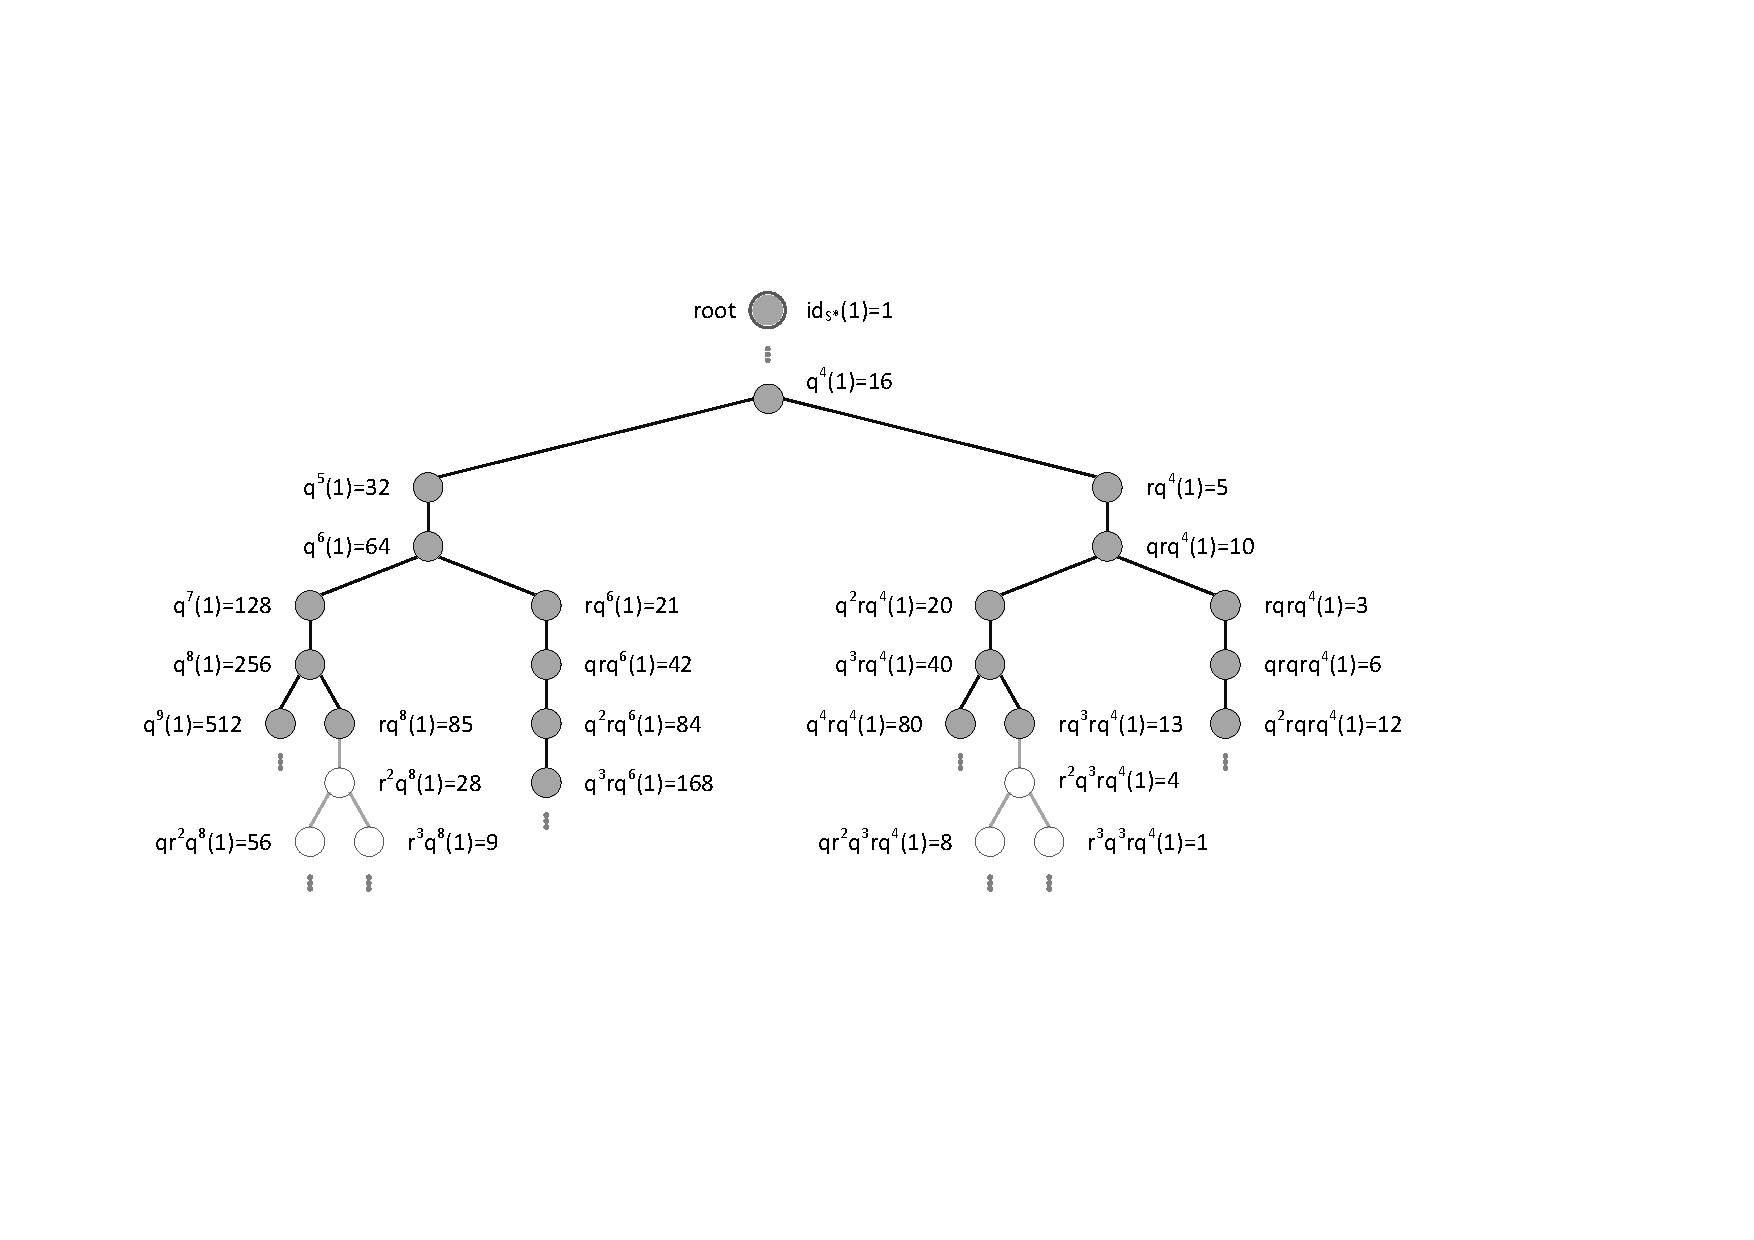
\includegraphics[trim=2.3cm 5.8cm 5.9cm 4.8cm, 
	width=1.00\textwidth,page=1]{figures/caytree.pdf}
	\caption{Small section of $H_T$ with darkly highlighted subtree $H_U$}
	\label{fig:1}
\end{figure}

\section{Defining the Tree}
The starting point for specifying our tree is $H_U$. Due to its
significance, we first concertize $H_U$ by the definition~\ref{def:H_U}
below, which establishes four essential characteristics.

\pagebreak
\begin{definition}
The graph $H_U$ possess the following key properties:
\begin{itemize}
	\item \mbox{\boldmath$H_U$} \textbf{is a directed graph (digraph):} Fundamentally, when we consider the more general case, an undirected graph as a triple $(V,E,\psi)$, the incidence function maps an edge to an arbitary vertex pair $\psi : E\rightarrow\{X\subseteq V:\left|X\right|=2\}$. In a digraph, the set $V\times V$ represents ordered vertex pairs. Accordingly the incidence function is more specifically defined, namely as a mapping of the edges to that set $\psi : E\rightarrow\{(v,w)\in V\times V:v\neq w\}$, see \cite[p.~15]{Ref_Korte_Vygen}.
	\item \mbox{\boldmath$H_U$} \textbf{is a rooted tree:} According to Rosen \cite[p.~747]{Ref_Rosen}, a rooted tree is "a tree in which one vertex has been designated as the root and every edge is directed away from the root." Peculiarly, this definition considers the directionality as an inherent part of rooted trees. Unlike Mehlhorn and Sanders \cite[p.~52]{Ref_Mehlhorn_Sanders}, for example, who distinguish between an undirected and directed rooted tree.
	\par\smallskip
	\textit{Note: As long as we do not stipulate that vertices may collapse, it is absolutely guaranteed that the graph is a tree.}
	\item \mbox{\boldmath$H_U$} \textbf{is an out-tree:} There is exactly one	path from the root to every other node \cite[p.~52]{Ref_Mehlhorn_Sanders}, which means that edge directions go from parents to children \cite[p.~108]{Ref_Du_Ko_Hu}. This property is implied in Rosen's definition for a rooted tree as well by saying "every edge is directed away from the root." An out-tree is sometimes designated as \textit{out-arborescence} \cite[p.~108]{Ref_Du_Ko_Hu}.
	\item \mbox{\boldmath$H_U$} \textbf{is a labeled tree:} For defining a labeled graph, Ehrig et al. \cite[p.~23]{Ref_Ehrig_etal} use a label alphabet consisting of a vertex label set and an edge label set. Since we only label the vertices, in our case the specification of a vertex label set $L_V$ together with the vertex label function $l_V:V\rightarrow L_V$ is sufficient. Originally, we said vertex labels are strings over the alphabet $S=\{q,r\}$, through which the free monoid $S^*$ is generated. We illustrate labeling $H_U$ by defining $l_{V(H_U)}(v)=ev^0_{S^*}(l_{V(G)}(\iota(v)),1)$, whereby $\iota:V(H_U)\hookrightarrow V(G)$ is the inclusion map \cite[p.~142]{Ref_Childs} from the set of vertices of $H_U$ to the set of vertices from the previously defined Cayley graph $G$.
\end{itemize}
\label{def:H_U}
\end{definition}

\par\medskip
We define a tree $H_C$ by taking the tree $H_U$ as a basis and for every
vertex $v\in V(H_U)$ satisfying $2\mid l_{V(H_U)}(v)$, we contract the
incoming edge. We attach the label of the parent of $v$ to the new
vertex, which results by replacing (merging) the two overlapping
vertices that the contracted edge used to connect. Visually, we
obtain $H_C$ by contracting all edges in $H_U$ that have an even-labeled 
target vertex, which (due to contraction) gets "merged into its parent." 
Edge contraction is occasionally referred to as \textit{collapsing an 
edge}. For more details and examples on edge contraction, one can see
Voloshin \cite[p.~27]{Ref_Voloshin} and Loehr \cite{Ref_Loehr}.

\par\medskip
The tree $H_C$ is a \textit{minor of $H_U$}, since it can be obtained
from $H_U$ "by a sequence of any vertex deletions, edge deletions and
edge contractions" \cite[p.~32]{Ref_Voloshin}. The sequence of contracting
the edges between adjacent (in our case even-labeled) vertices is called
\textit{path contraction}.

\par\medskip
A small section of the tree $H_C$ is shown in figure~\ref{fig:2}. Other
definitions of the same tree exist, see for example Conrow 
\cite{Ref_Conrow} or Bauer \cite[p.~379]{Ref_Bauer}.

\begin{figure}
	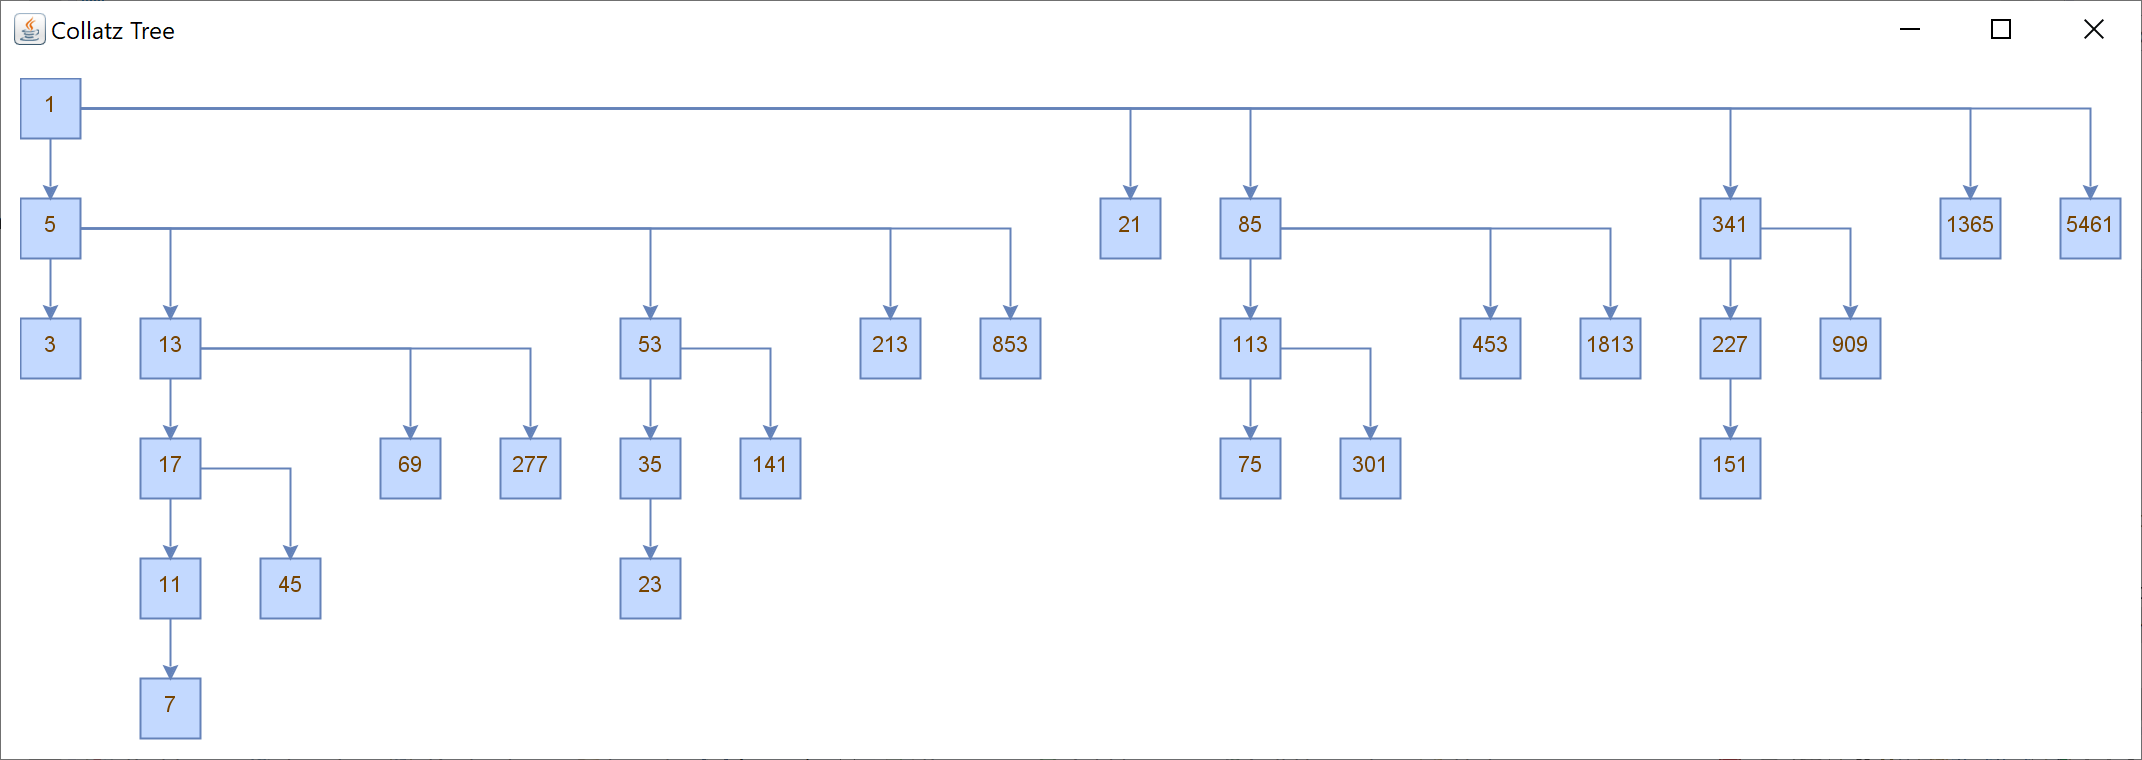
\includegraphics[width=1.00\textwidth]{figures/h_c.png}
	\caption{Small section of $H_C$ (displaying the trivial cycle is waived)}
	\label{fig:2}
\end{figure}

\section{Relationship of successive nodes in \mbox{$H_C$}}

Let $v_1$ and $v_{1+n}$ be two vertices of $H_C$, where $v_1$ is
reachable from $v_{1+n}$ with $level(v_1)-level(v_{1+n})=n$.
Hence, a path $(v_{1+n},\ldots,v_1)$ exists between these two
vertices. Theorem~\ref{theo:1} specifies the following relationship
between $v_1$ and $v_{1+n}$.

\par\medskip
\begin{theorem}
	\label{theo:1}
	$l_{V(H_C)}(v_{1+n})=3^nl_{V(H_C)}(v_1)\prod_{i=1}^{n}\left(1+\frac{1}{3l_{V(H_C)}(v_{i})}\right)2^{-\alpha_i}$.
	In order to simplify readability, we waive writing down the vertex label function and put it shortly:\\
	$v_{1+n}=3^nv_1\prod_{i=1}^{n}\left(1+\frac{1}{3v_{i}}\right)2^{-\alpha_i}$.
	The value $\alpha_i\in\mathbb{N}$ is the number of edges which have been contracted between $v_i$ and $v_{i+1}$ in $H_U$.
\end{theorem}

In order to demonstrate the construction produced by theorem~\ref{theo:1} in an illustrative fashion, example~\ref{ex:vertices} runs through a concrete path in $H_C$.

\par\medskip
\begin{example}
	\label{ex:vertices}
	For example, the two vertices $v_1=45$ and $v_{1+3}=v_4=5$ are 
	connected
	via the path $(5,13,17,45)$, see figure~\ref{fig:2}. Furthermore, one
	can retrace in figure~\ref{fig:3} the uncontracted path between these
	two nodes within $H_U$. When applied to this example,
	theorem~\ref{theo:1} produces the following:	
	\begin{center}
		$5=v_{1+3}=3^3*45*\left(1+\frac{1}{3*45}\right)*2^{-3}
		*\left(1+\frac{1}{3*17}\right)*2^{-2}
		*\left(1+\frac{1}{3*13}\right)*2^{-3}$
	\end{center} 
\end{example}
\begin{proof}
	\label{proof:1}
	This relationship of successive nodes can simply be proven inductively. For the base case, we set $n=1$ and retrieve
	\begin{center}
		$v_{1+1}=3v_1\left(1+\frac{1}{3v_1}\right)2^{-\alpha_1}
		=\left(3v_1+1\right)2^{-\alpha_1}=v_2$
	\end{center}
	The path from $v_2$ to $v_1$ can conformly be expressed by a string $rq\cdots q$ of $S^*$, because of $v_1=r\circ q^{\alpha_1}\left(v_2\right)$. We set $n=n+1$ for the step case, which leads to
	\begin{equation*}
	\begin{array}{cl}
	v_{n+2} &
	=3^{n+1}v_1\prod_{i=1}^{n+1}\left(1+\frac{1}{3v_i}\right)2^{-\alpha_i}\\
	&
	=3^{n+1}v_1\left(1+\frac{1}{3v_{n+1}}\right)2^{-\alpha_{n+1}}\prod_{i=1}^{n}\left(1+\frac{1}{3v_i}\right)2^{-\alpha_i}\\
	&
	=3\left(1+\frac{1}{3v_{n+1}}\right)2^{-\alpha_{n+1}}3^nv_1\prod_{i=1}^{n}\left(1+\frac{1}{3v_i}\right)2^{-\alpha_i}\\
	&
	=3\left(1+\frac{1}{3v_{n+1}}\right)2^{-\alpha_{n+1}}v_{1+n}\\
	&
	=\left(3v_{1+n}+1\right)2^{-\alpha_{n+1}}
	\end{array}
	\end{equation*}
	In this case the path from $v_{n+2}$ to $v_{n+1}$ is conformly 
	expressable by a string $rq\cdots q$ of $S^*$ too, since
	$v_{n+1}=r\circ q^{\alpha_{n+1}}\left(v_{n+2}\right)$.
\end{proof}

Even though the tree may theoretically contain two or more identically labeled vertices, it is essential to emphasize that we only consider such paths $(v_{1+n},\ldots,v_1)$ whose vertices are all labeled differently. Later in section~\ref{sec:cycles}, we even require that identically labeled nodes are one and the same. In order to get correct results using Theorem~\ref{theo:1} we specify its halting conditions by definition~\ref{def:halting_condition}.

\begin{definition}
	\label{def:halting_condition}
	When determining successive nodes starting at $v_1$ according to Theorem~\ref{theo:1}, we halt if one of the following two conditions is fulfilled:
	\begin{enumerate}
		\item $v_{n+1}=1$
		\item $v_{n+1}\in\{v_1,v_2,\ldots,v_n\}$
	\end{enumerate}
	If the first condition applies, the Collatz conjecture is true for a specific sequence. When the second condition is fulfilled, the sequence has led to a cycle. For every starting node, except the root node (labeled with $1$), the Collatz conjecture is consequently falsified. Let us consider the example $v_1=13$, where the algorithm halts after two iterations, because after two iterations the first condition holds:
	\[
	v_{1+n}=3^2\cdot\left(1+\frac{1}{3\cdot13}\right)\left(1+\frac{1}{3\cdot5}\right)\cdot2^{-7}=1
	\]
	
	If we examine the case $v_{1}=1$, we realize that the algorithm finishes after the first iteration, since both halting conditions become true. The sequence stops because the final node labeled with $1$ is reached after one iteration. Furthermore the sequence has led to a cycle:
	\[
	v_{1+n}=3\cdot\left(1+\frac{1}{3}\right)2^{-2}=1
	\]
	
	As the latter example shows, the trivial cycle is the only sequence where both conditions are fulfilled.
\end{definition}

\noindent
Theorem~\ref{theo:1} can be used for specifying the condition of a cycle as follows:

\begin{equation}
\label{eq:func_cycle}
\begin{array}{l}
v_{1}=3^nv_1\prod_{i=1}^{n}\left(1+\frac{1}{3v_i}\right)2^{-\alpha_i}
\\[\medskipamount]
2^{\alpha_1+\cdots+\alpha_n}=\prod_{i=1}^{n}\left(3+\frac{1}{v_i}\right)
\end{array}
\end{equation}

A similar condition has been formulated by Hercher \cite{Ref_Hercher}. Taking a first look at equation~\ref{eq:func_cycle}, we are able to recognize the trivial cycle for $n=1$. One might easily come to the false conclusion that the term only results in a natural number for this trivial cylce, since we are multiplying fractions. The following counterexample, starting at $v_1=31$, disproves this assumption:
\begin{equation*}
20480=\left(3+\frac{1}{31}\right)\left(3+\frac{1}{47}\right)
\left(3+\frac{1}{71}\right)\left(3+\frac{1}{107}\right)\left(3+\frac{1}{161}\right)\left(3+\frac{1}{121}\right)\left(3+\frac{1}{91}\right)\left(3+\frac{1}{137}\right)\left(3+\frac{1}{103}\right)
\end{equation*}

According to OESIS \cite{Ref_OESIS}, the integer $v_1=31$ is called \textit{self-contained}. The term self-contained is based on the fact that the node $v_{n+1}=v_{10}=155$ is divisible by the starting node $v_1=31$ and $v_{10}$ results from applying one and the same function (in this case the Collatz function) using $v_1$ as input, see also Guy \cite[p.~332]{Ref_Guy}. For such a case equation~\ref{eq:func_cycle} leads to a natural number, but not necessarily to a cycle. A cycle only occurs if the term results in a power of two. One example is the trivial cycle. We find another case if we choose the factor $5$ instead of $3$:
\begin{center}
	$128=2^7=\left(5+\frac{1}{13}\right)\left(5+\frac{1}{33}\right)
	\left(5+\frac{1}{83}\right)$
\end{center}

The above example shows that non-trivial cycles can be found if we generalize the Collatz conjecture by replacing the factor $3$ with the variable $k$. We study this generalized form and the occurance of cycles in chapter \ref{sec:cycles} more deeply. A detailed elaboration of the divisibility and a deeper understanding of the tree $H_C$ needs to be performed in order to get towards any proof of the Collatz conjecture.

%\par\medskip\noindent
%Generally, for any variant $kx+1$ it applies that if $v_1\mid v_{n+1}$, the the product is natural:
%\begin{equation*}
%	\prod_{i=1}^n\left(k+\frac{1}{v_i}\right)\in \mathbb{N}
%\end{equation*}

\begin{figure}
	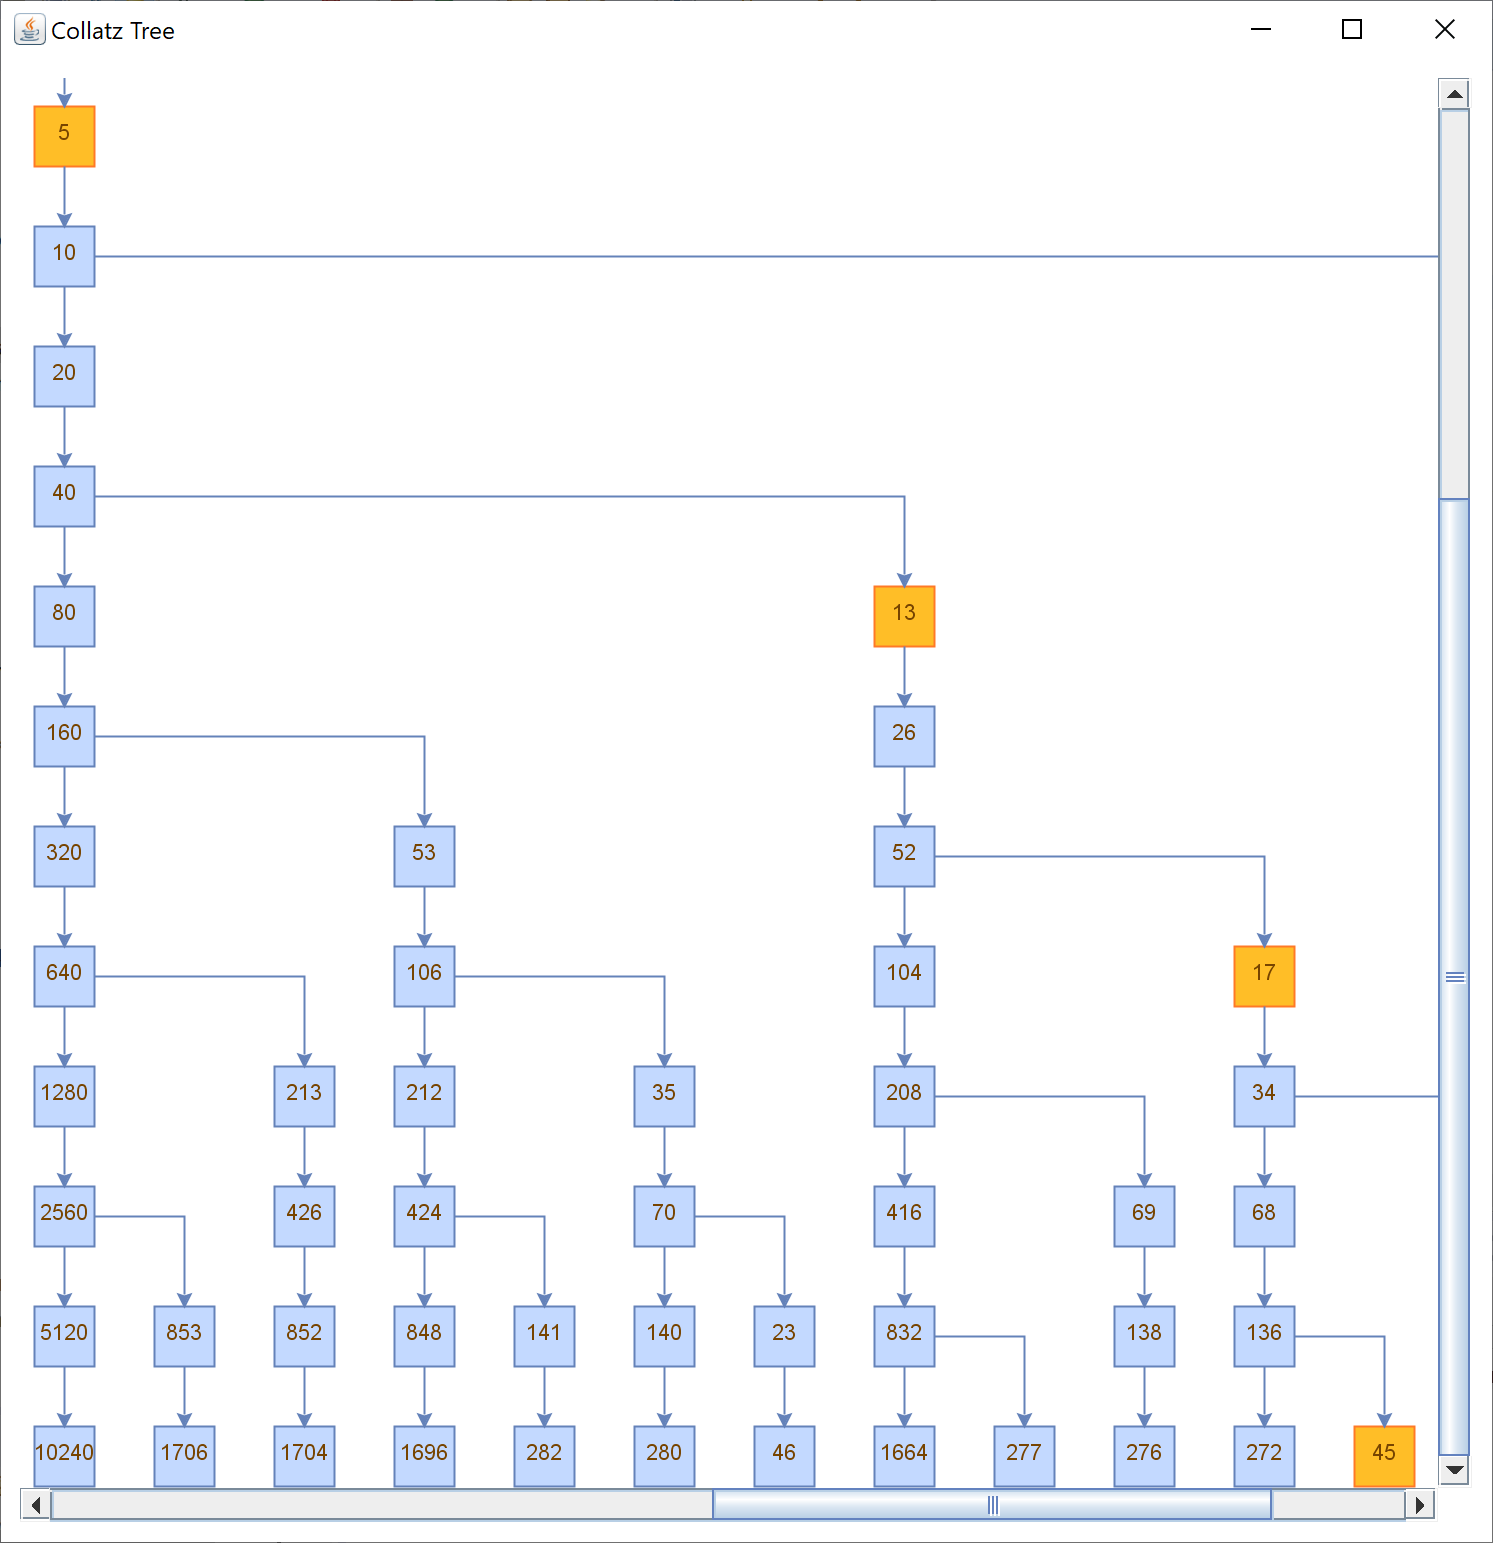
\includegraphics[width=1.00\textwidth]{figures/h_u.png}
	\caption{Section of $H_U$ containing the path from $5$ to $45$}
	\label{fig:3}
\end{figure}

\section{Relationship of sibling nodes in \mbox{$H_C$}}
In a rooted tree, vertices which have the same parent are called "siblings" \cite[p.~702]{Ref_Johnsonbaugh}, \cite[p.~747]{Ref_Rosen}. Sibling vertices accordingly have the same level.

\par\medskip
Let $w$ be a vertex, from which a path exists to the vertex $v_1$. Let $v_2$ be the immediate right-sibling of $v_1$, then $l_{V\left(H_C\right)}\left(v_2\right)=4*l_{V\left(H_C\right)}\left(v_1\right)+1$. This fact has been expressed differently by Kak \cite{Ref_Kak_2014} as follows: "If an odd number $a$ leads to another odd number (after several applications of the Collatz transformation) $b$, then $4a+1$ also leads to $b$."

\par\medskip
Applied to our approach, consider $w$ as the parent of $v_1$ and $v_2$. Suppose, in $H_U$, a path consisting of $n+1$ edges goes from $w$ to $v_1$. Then we can straightforwardly show that $n$ edges in $H_U$ have been contracted between both nodes $w$ and $v_1$ and $n+2$ edges between $w$ and $v_2$ (for simplicity we again omit writing the label function):
\begin{equation*}
\begin{array}{l}
		v_1=\frac{w*2^n-1}{3}
		\\[\medskipamount]
		v_2=\frac{w*2^{n+2}-1}{3}=4*v_1+1
\end{array}
\end{equation*}

For example, $n=3$ edges in $H_U$ have been contracted between $w=5$ and $v_1=13$ and $n+2=5$ edges between $w$ and $v_2=53$, whereby in $H_C$, the vertex $v_2$ is the right-sibling of $v_1$ and these two sibling vertices are immediate children of $w$.

\section{A vertex's \mbox{$n$}-fold left-child and right-sibling in \mbox{$H_C$}}
Referring to the "left-child, right-sibling representation" of rooted trees \cite[p.~246]{Ref_Cormen_Leiserson_Rivest_Stein}, the function $\textit{left-child}:V\rightarrow V$ returns the leftmost child of a vertex $v$. Nesting this function $n$ times leads to the definition of a vertex's $n$-fold left-child, which is given by $\textit{left-child}^n(v)$. As shown in figure~\ref{fig:2}, for example $\textit{left-child}^3(13)=7$.

\par\medskip
The function $\textit{right-sibling}:V\rightarrow V$ points to the sibling of a vertex $v$ immediately to its right \cite[p.~246]{Ref_Cormen_Leiserson_Rivest_Stein}. If this function is nested $n$ times, we get a vertex's $n$-fold right-sibling defined by $\textit{right-sibling}^n(v)$. One example is $\textit{right-sibling}^2(113)=1813$ which has been demonstrated in figure~\ref{fig:2} too.

\par\medskip
Let $w$ be a vertex in $H_C$ and $v_0$ the left-child of $w$. The $n$-fold right-sibling of $v_0$ can be calculated as follows:
\begin{equation}
\label{eq:nfold_right_sibling}
	v_n=\textit{right-sibling}^n(v_0)=\frac{1}{3}*\left(w*2^{2*n+\pi_3(w\bmod 3)}-1\right)
\end{equation}

The function $\pi_3$ is the self-inverse permutation (involution):
\begin{equation}
\label{eq:pi_3}
	\pi_3=\left(\begin{array}{cc}
	1 & 2\\
	2 & 1
	\end{array}\right)
\end{equation}
We consider permutations of the set $\{1,2\}$ and not of $\{0,1,2\}$, due to the fact that $w\bmod 3$ cannot be zero. A node $w$ in $H_C$, which is labeled by an integer divisible by $3$ is a leaf; and therefore such node has no left-child, more specifically it has no children at all.

\par\medskip
\noindent
When setting $n=0$, we trivially retrieve the vertex's $w$ left-child:
\begin{center}
	$v_0=\textit{left-child}(w)=\frac{1}{3}*\left(w*2^{\pi_3(w\bmod 3)}-1\right)$
\end{center}

\begin{example}
	\label{ex:siblings}
	Let us refer to figure~\ref{fig:2} again and pick out $w=5$. Then the
	vertex's $w$ left-child is $v_0=3$ and the threefold right-sibling
	$v_3=213$:

	\begin{equation*}
	\begin{array}{l}
		v_0=\frac{1}{3}*\left(5*2^{\pi_3(5\bmod 3)}-1\right)=3
		\\[\medskipamount]
		v_3=\frac{1}{3}*\left(5*2^{2*3+\pi_3(5\bmod 3)}-1\right)=213
	\end{array}
	\end{equation*}
\end{example}

\section{Left-child and right-sibling in the \mbox{$5x+1$} variant of \mbox{$H_C$}}
In the following we take a look at the $5x+1$ variant of $H_C$. We name this graph $H_{C,5}$ and must note that it is not a tree and moreover that not all of its vertices are reachable from the root. We define the permutation $\pi_5$ as follows:
\begin{center}
	$\pi_5=\left(\begin{array}{cccc}
		1 & 2 & 3 & 4\\
		4 & 3 & 1 & 2
	\end{array}\right)$	
\end{center}

Next, by letting $w$ be a vertex in $H_{C,5}$ and $v_0$ the left-child of $w$
we obtain the $n$-fold right-sibling of $v_0$ by the function that
is slightly different to the one defined by \ref{eq:nfold_right_sibling}:
\begin{equation}
\label{eq:nfold_right_sibling_5}
	v_n=\textit{right-sibling}^n(v_0)=\frac{1}{5}*\left(w*2^{4*n+\pi_5(w\bmod 5)}-1\right)
\end{equation}

Analogous to \ref{eq:pi_3} only permutations on the set without zero
\{1,2,3,4\} need to be considered, since $w\bmod 5$ cannot be zero.
Otherwise, if $w\equiv 0 (\bmod 5)$ which means that $w$ were labeled
by an integer divisible by 5, then the node $w$ has no successor in $H_{C,5}$.

\par\medskip
\noindent
By setting $n=0$, the function (above given by \ref{eq:nfold_right_sibling_5}) returns the left child of $w$:
\begin{center}
	$v_0=\textit{left-child}(w)=\frac{1}{5}*\left(w*2^{\pi_5(w\bmod 5)}-1\right)$
\end{center}

\begin{figure}
	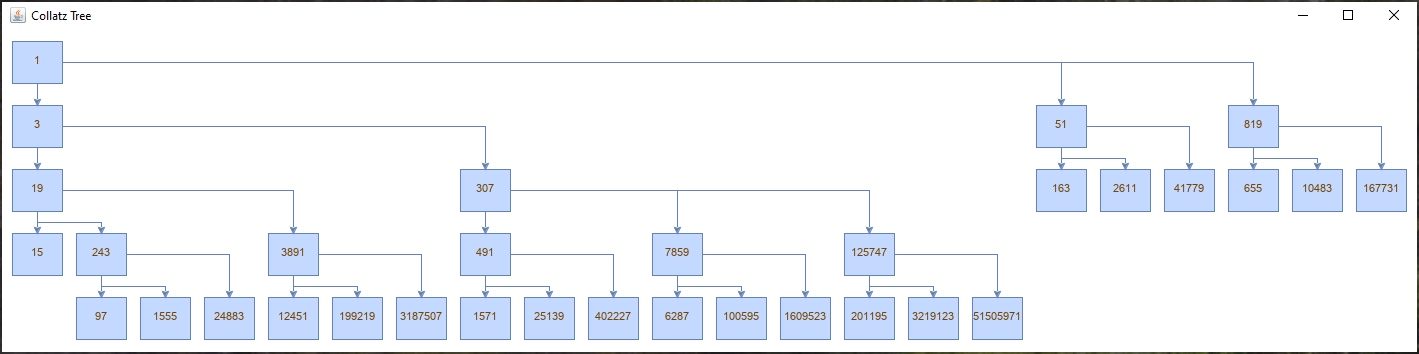
\includegraphics[width=1.00\textwidth]{figures/h_c5b.png}
	\caption{Section of the graph $H_{C,5}$ starting at its root (without branches that reflect a subsequence containing the trivial cycle)}
	\label{fig:4}
\end{figure}

Figure~\ref{fig:4} illustrates a small section of $H_{C,5}$ starting at its root. The particularly interesting thing about the graph $H_{C,5}$ is that it contains three cycles, the trivial cycle starting from the root $1,3$ and two non-trivial cycles $43,17,27$ and $83,33,13$. To be precise, three cycles are known (as it will become apparent later in section~\ref{sec:non_trivial_cycles}), and on the basis of present knowledge it cannot be ruled out with any certainty that other cycles exist.

\section{A remark about cycles}
\label{sec:cycles}
In graph theory, a path of length $n\geq 1$ that starts and ends at the same vertex is called a circuit. A circuit, in which no vertex is repeated with the sole exception that the initial vertex is the terminal vertex, is called a cycle. A cycle of length $n$ is referred to as an $n$-cycle. For these definitions, we rely on \cite[p.~599]{Ref_Rosen}, \cite[p.~35]{Ref_Benjamin_Chartrand_Zhang} and \cite[p.~445]{Ref_Chartrand_Zhang}. Furthermore, we call a cycle originating from the root a trivial cycle.

\begin{remark}
In order for the cycles to become graphically visible, we now require that in a graph $H$ two vertices $v_1$ and $v_2$ are one and the same if the label of both nodes are identical: $l_{V(H)}(v_1)=l_{V(H)}(v_2)\rightarrow v_1=v_2$. As a consequence, there is no guarantee that the graph precisely refers to the algebraic structure of a free monoid anymore. A free monoid requires that each of its elements can be written in one and only one way.
\end{remark}

When different nodes collapse on one, the graph is no longer necessarily a tree. Let us point to the monoid S*, which we introduced in section \ref{sec:groups_graphs}. Take for example four of its elements, the empty string $e$, the strings $qqr$, $qqrqqr$, and $qqrqqrqqr$. These elements lie as well within the subset $U\subset T\subset S^*$, and they are represented by nodes of the tree $H_U$ that all have the same label $1=ev_{S^*}(qqr,1)=ev_{S^*}(qqrqqr,1)=ev_{S^*}(qqrqqrqqr,1)$. These nodes are one and the same, the root of $H_U$. Visually, then in $H_U$ a directed edge goes from the vertex labeled with $4$ back to the root node. Analogically, in $H_C$ a loop connects the root to itself, since due to the path contraction even labeled nodes do not exist in $H_C$. The  aforementioned example reflects the trivial cycle of the Collatz sequence.

\par\medskip
Figure~\ref{fig:5} depicts a section of $H_{C,5}$, which includes the $3$-cycle $43,17,27$. Because of the two non-trivial cycles $43,17,27$ and $83,33,13$, in $H_{C,5}$ there does not exist a path between the root and the vertex $43$ and between the root and the vertex $83$. Hence, $H_{C,5}$ is said to be a disconnected graph. Generally, a graph is called a disconnected graph if it is impossible to walk (along its edges) from any vertex to any other \cite[pp.~46-47]{Ref_Benjamin_Chartrand_Zhang}.

\begin{figure}
	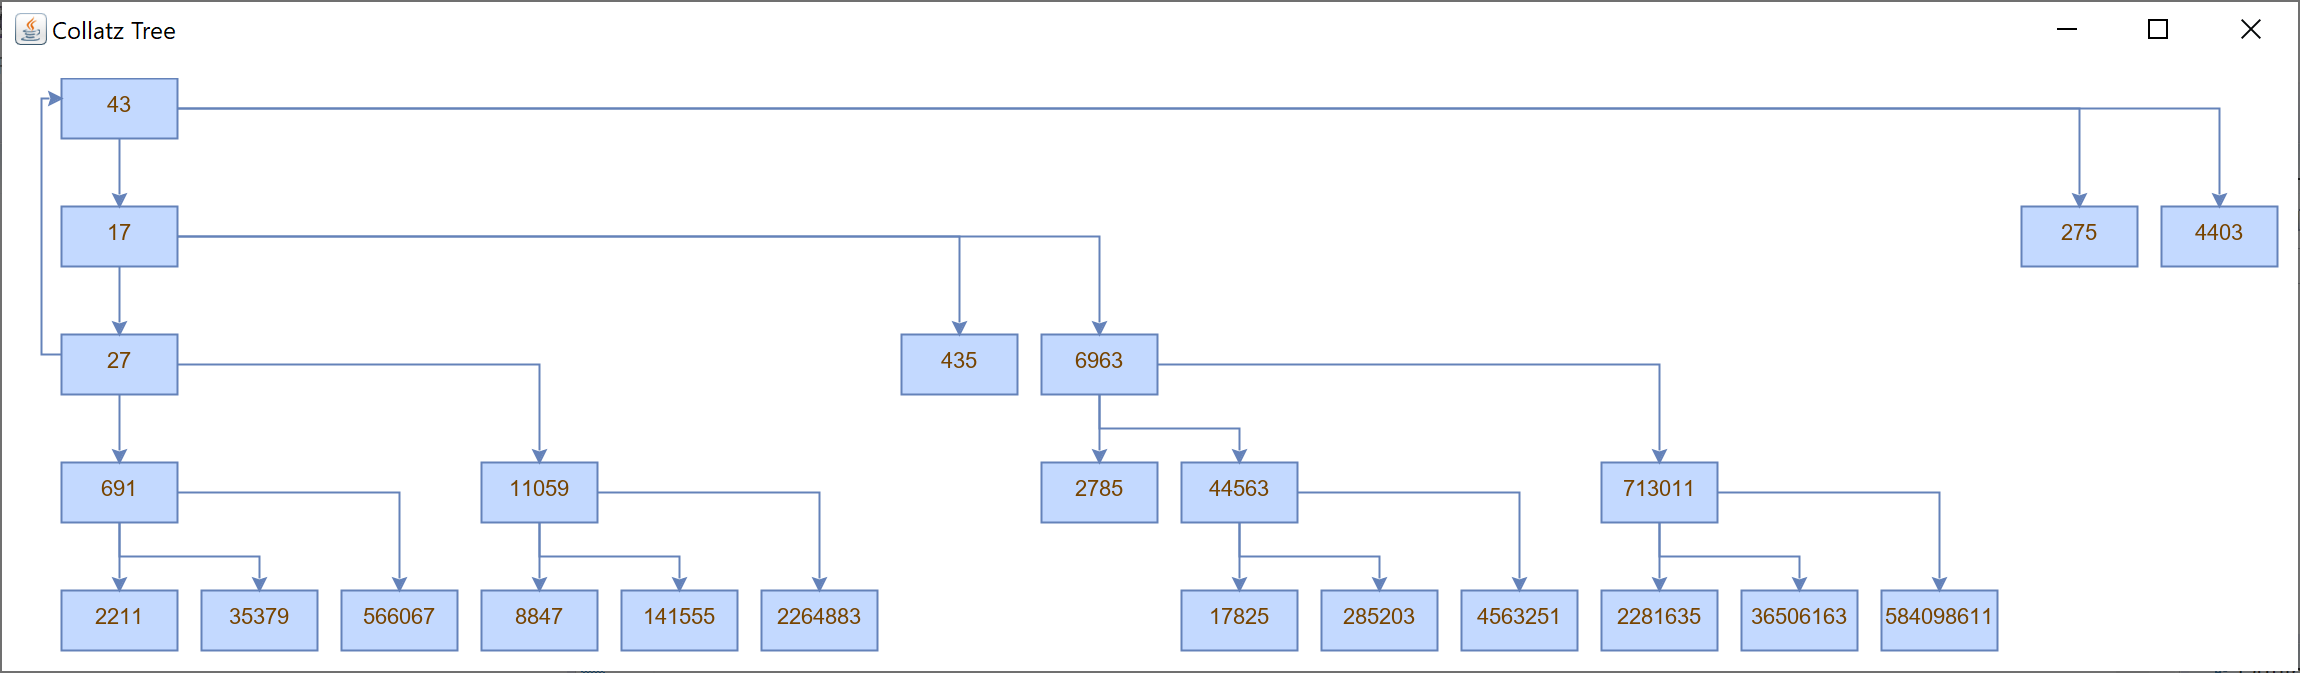
\includegraphics[width=1.00\textwidth]{figures/h_c5a.png}
	\caption{Section of $H_{C,5}$ including the $3$-cycle $43,17,27$}
	\label{fig:5}
\end{figure}

\par\medskip
The following considerations focus on non-trivial cycles, and therefore on cycles that do not originate from the root, but cause the graph to be a disconnected graph. Utilizing the example of the graph $H_{C,5}$ we are able to deduct from the cycle $43,17,27$ the simple and self-evident equality $\textit{left-child}^3(43)=43$:
\begin{equation*}
	\begin{array}{l}
		\textit{left-child}(43)=\frac{1}{5}*\left(43*2^1-1\right)=17
		\\[\medskipamount]
		\textit{left-child}(17)=\frac{1}{5}*\left(17*2^3-1\right)=27
		\\[\medskipamount]
		\textit{left-child}(27)=\frac{1}{5}*\left(27*2^3-1\right)=43
	\end{array}
\end{equation*}

Obviously, the authors note, it would be interesting to find out what circumstances enable a graph to have non-trivial cycles, whether it be the $5x+1$ variant of $H_C$, the $7x+1$ variant of $H_C$ or any variant of $H_C$; let us say the $kx+1$ variant of $H_C$ with $k\geq 1$.

\section{Which variants of \mbox{$H_C$} have non-trivial cycles?}
\label{sec:non_trivial_cycles}
Let us refer to a $kx+1$ variant of $H_C$ as $H_{C,k}$. By having introduced and proven theorem~\ref{theo:1} we already started an assertion about the reachability of successive nodes in $H_C$. This reachability relationship can be generalized for any graph $H_{C,k}$ as follows:
\begin{equation}
\label{eq:generalized_reachability}
v_{1+n}=k^nv_1\prod_{i=1}^{n}\left(1+\frac{1}{kv_{i}}\right)2^{-\alpha_i}
\end{equation}

This generalization leads to the condition for an existence of an $n$-cycle in any $kx+1$ variant of $H_C$, which looks analogous to the condition given by equation~\ref{eq:func_cycle} that specifies $H_C$ has a cycle:
\begin{equation}
\label{eq:generalized_cycle}
2^\alpha=\prod_{i=1}^{n}\left(k+\frac{1}{v_i}\right)
\end{equation}

The natural number $\alpha$ is the sum of edges that have been contracted between the vertices $v_i$ forming the cycle, in other words $\alpha$ is the number of divisions by $2$ within the sequence. The natural number $n$ is the cycle length and $k$ obviously specifies the variant of $H_C$. Since between each vertex at least one edge has been contracted (at least one division by $2$ took place), we know that our exponent alpha is greater than or equal to the sequence length:
\begin{equation}
\label{eq:n_alpha}
	\alpha\ge n
\end{equation}

\par\medskip
Using incremental search, one can calculate cycles through trial and error. Table~\ref{table:known_cycles} lists all empirically discovered cycles having a length up to $100$ that appear in $kx+1$ variants of $H_C$ for $k\in[1,1000]$. Within each of these variants, the cycles have been searched at potential starting nodes $v_1$ with a label between $1$ and $1000$. Note that the cycles in table~\ref{table:known_cycles} are written in reverse order, i.e. in the order which corresponds to the Collatz sequence. To obtain the cycles in terms of graph theory referring to the graph $H_C$, read them from right to left.

\begin{table}[H]
	\centering
	\begin{tabular}{|L{2cm}|R{4cm}|R{2cm}|C{2cm}|}
		\hline
		\thead{\boldsymbol{$k$}} &
		\thead{\textbf{cycle}} &
		\thead{\boldsymbol{$\alpha$}} &
		\thead{\textbf{non-trivial}} \\
		\hline
		1 &
		1 &
		1 &
		\\
		\hline
		3 &
		1 &
		2 &
		\\
		\hline
		5 &
		1,3 &
		5 &
		\\
		\hline
		5 &
		13,33,83 &
		7 &
		\checkmark \\
		\hline
		5 &
		27,17,43 &
		7 &
		\checkmark \\
		\hline
		7 &
		1 &
		3 &
		\\
		\hline
		15 &
		1 &
		4 &
		\\
		\hline
		31 &
		1 &
		5 &
		\\
		\hline
		63 &
		1 &
		6 &
		\\
		\hline
		127 &
		1 &
		7 &
		\\
		\hline
		181 &
		27,611 &
		15 &
		\checkmark \\
		\hline
		181 &
		35,99 &
		15 &
		\checkmark \\
		\hline
		255 &
		1 &
		8 &
		\\
		\hline
		511 &
		1 &
		9 &
		\\
		\hline
	\end{tabular}
	\caption{Known $n$-cycles in $kx+1$ variants of $H_C$ for $k\leq1000$, $n\leq 100$}
	\label{table:known_cycles}
\end{table}

Based on the results shown in table~\ref{table:known_cycles} we state the following theorem~\ref{theo:2} that renders more precisely the prerequisite for cycles that may occur in variants of $H_C$.

\par\medskip
\begin{theorem}
\label{theo:2}
An $n$-cycle can only exist in a graph $H_{C,k}$, that means in a $kx+1$ variant of $H_C$, if the following equation holds:
\begin{equation*}
2^{\bar\alpha}=2^{\lfloor n\log_2k\rfloor+1}=\prod_{i=1}^{n}\left(k+\frac{1}{v_i}\right)
\end{equation*}
\end{theorem}

\par\medskip
The key of theorem~\ref{theo:2} consists in the claim that, in order for an $n$-cycle to occur, the exponent $\alpha$ has to be $\bar\alpha=\lfloor n\log_2k\rfloor+1$. We approach a proof by expressing formally that $\bar\alpha$ is not allowed to be smaller and it is not allowed to be greater than $\lfloor n\log_2k\rfloor+1$, in other words we indicate a lower and an upper limit for $\bar\alpha$ as follows:

\begin{samepage}
	\begin{flalign}
		\label{eq:inequality_min}
		&\bar\alpha>\lfloor n\log_2k\rfloor\\	
		\label{eq:inequality_max}
		&\bar\alpha<\lfloor n\log_2k\rfloor+2
	\end{flalign}
\end{samepage}

The validity of the first part (\ref{eq:inequality_min}), which specifies $\lfloor n\log_2k\rfloor+1$ as the lower limit for $\bar\alpha$, can be demonstrated in a fairly simple way: Our starting point is equation~\ref{eq:generalized_reachability}, which describes the relationship of successive vertices in $H_{C,k}$. Having a cycle, requires us to consider the first and the last vertex being one and the same $v_{1+n}=v_1$. Setting a smaller exponent $\bar\alpha=\lfloor n\log_2k\rfloor$ into equation~\ref{eq:generalized_reachability} results in the inequality $v_{1+n}>v_1$, which is in any case a true statement:
\begin{equation*}
	\begin{array}{l}
		k^nv_12^{-\lfloor n\log_2k\rfloor}\prod_{i=1}^{n}\left(1+\frac{1}{kv_{i}}\right)>v_1
		\\[\medskipamount]
		k^n\prod_{i=1}^{n}\left(1+\frac{1}{kv_{i}}\right)>2^{\lfloor\ nlog_2k\rfloor}
		\\[\medskipamount]
		\log_2\left(k^n\prod_{i=1}^{n}\left(1+\frac{1}{kv_{i}}\right)\right)>\lfloor n\log_2k\rfloor
		\\[\medskipamount]
		n\log_2k+log_2\left(\prod_{i=1}^{n}\left(1+\frac{1}{kv_{i}}\right)\right)>\lfloor n\log_2k\rfloor
	\end{array}	
\end{equation*}

The validity of the second part (\ref{eq:inequality_max}) is not so trivial to prove. Analogous to the above-shown proof of alpha's lower limit, we again refer to equation~\ref{eq:generalized_reachability} as our starting point and we need to show that $v_{1+n}$ is smaller than $v_1$ if $\alpha=\lfloor\ nlog_2k\rfloor+2$:
\begin{equation*}
	\begin{array}{l}
		k^nv_12^{-\left(\lfloor n\log_2k\rfloor+2\right)}\prod_{i=1}^{n}\left(1+\frac{1}{kv_{i}}\right)<v_1
		\\[\medskipamount]
		k^n\prod_{i=1}^{n}\left(1+\frac{1}{kv_{i}}\right)<2^{\left(\lfloor n\log_2k\rfloor+2\right)}
	\end{array}	
\end{equation*}
This leads to the following general condition for the validity of alpha's upper limit:
\begin{equation}
\label{eq:condition_max}
	n\log_2k-\lfloor n\log_2k\rfloor<2-log_2\left(\prod_{i=1}^{n}\left(1+\frac{1}{kv_{i}}\right)\right)
\end{equation}

A product $\prod(1+a_n)$ with positive terms $a_n$ is convergent if the series $\sum a_n$ converges, see Knopp \cite[p.~220]{Ref_Knopp}. Thus, to verify whether the product in condition~\ref{eq:condition_max} is converging towards a limiting value, it is sufficient to examine the following sum:
\begin{equation*}
\sum_{i=1}^{n}\frac{1}{kv_{i}}
\end{equation*}

We write down the successive vertices and obtain:
\begin{flalign*}
	v_1&=v_1\\
	v_2&=\frac{kv_1+1}{2^{\alpha_1}}\\
	v_3&=\frac{k^2v_1+k+2^{\alpha_1}}{2^{\alpha_1+\alpha_2}}\\
	v_4&=\frac{k^3v_1+k^2+k\cdot2^{\alpha_1}+2^{\alpha_1+\alpha_2}}{2^{\alpha_1+\alpha_2+\alpha_3}}\\
	\vdots\\
	v_{n+1}&=\frac{k^nv_1+\sum_{j=1}^{n}k^{j-1}2^{\alpha_1+\ldots+\alpha_n-\sum_{l>n-j}\alpha_l}}{2^{\alpha_1+\ldots+\alpha_n}}
\end{flalign*}

For the sum of the reciprocal vertices we have the following: 
\begin{equation*}
\sum_{i=1}^{n+1}\frac{1}{kv_i}=\frac{1}{k}\left(\frac{1}{v_1}+\sum_{i=1}^{n}\frac{1}{v_{i+1}}\right)=\frac{1}{k}\left(\frac{1}{v_1}+\sum_{i=1}^{n}\frac{2^{\alpha_1+\ldots+\alpha_i}}{k^iv_1+\sum_{j=1}^{i}k^{j-1}2^{\alpha_1+\ldots+\alpha_n-\sum_{l>i-j}\alpha_l}}\right)
\end{equation*}

\section{Existence of a solitary cycle for $k=1$}
As per theorem~\ref{theo:2}, for $k=1$, the only possible alpha for a cycle is $1$:
\[
\bar\alpha=\lfloor n\log_21\rfloor+1=1
\]
In accordance with the condition $\alpha\ge n$ stated by \ref{eq:n_alpha} it is clear that between two successive vertices at least one edge has been contracted or respectively one division by two took place. This exactly is the reason why, if theorem~\ref{theo:2} is true, a cycle can only occur for $n=1$. Based on equation~\ref{eq:generalized_cycle} we can show that this is the case for the trivial cycle, starting at the root $v_1=1$:
\[
2^{\bar\alpha}=2^{\lfloor 1\log_21\rfloor+1}=2^1=\left(1+\frac{1}{v_1}\right)=\left(1+\frac{1}{1}\right)
\]
Since no other value of $v_1$ results in a natural number, no other cycle for $n=1$ is possible. In order to prove theorem~\ref{theo:2} for $k=1$, we now have to show that condition~\ref{eq:condition_max} is true.

\section{Verifying alpha's upper limit for the $1x+1$ variant of $H_C$}
We prove that theorem~\ref{theo:2} is true for $k=1$ using the so-called Engel expansion, which we will explore more closely later in section~\ref{sec:worstcase_k3}. Setting $b=2$ and $k=1$ into equation~\ref{eq:generalized_asc_continued_fraction} leads to the formula that calculates the node $v_{n+1}$ for a sequence, in which we divide by $2$ only once per iteration:
\begin{equation}
\label{eq:appx_1}
v_{n+1}=\frac{v_1+2^n-1}{2^n}
\end{equation}

\begin{example}
	Let us consider the sequence $v1=17$, $v_2=9$, $v_3=5$, $v_4=3$. Setting $v_1=17$ and $n=3$ results in:
	\[
	v_{3+1}=v_4=\frac{17+2^3-1}{2^3}=3
	\]
\end{example}

Equation~\ref{eq:appx_1} represents the (hypothetical) case in which a sequence progresses to the highest possible successive node for a specific starting node $v_1$. Actually, the sequence decreases in any case except $v_1=1$ and $n=1$. We can show that setting $v_1=1$ and $n=1$ results in the trivial cycle:
\[
v_1=1=v_2=\frac{1+2^1-1}{2^1}
\]

The equation above, complies to (and verifies) theorem~\ref{theo:2}, since $1=n=\alpha=\bar\alpha$:
\[
\bar\alpha=\lfloor n*log_21\rfloor+1=1
\]

The condition~\ref{eq:n_alpha}, namely the inequality $\alpha\ge n$, can be used to prove that no other $\alpha$ than $\bar\alpha$ leads to a cycle. To show this, we set $v_{n+1}=v_1$:
\[
v_1=\frac{v_1+2^n-1}{2^n}=\frac{v_1}{2^n}-\frac{1}{2^n}+1=\frac{v_1-1}{2^n}+1
\]

The above term is only true for $v_1=1$ and $n=\alpha=\bar\alpha=1$. Any higher value for $v_1$, $n$ or $\alpha$ leads to a result less than $v_1$. Therefore, a cycle is not possible for $\alpha\ne 1$ and theorem~\ref{theo:2} is true for $k=1$. A cycle can only occur for the case $v_1=1$ and $\alpha=\bar\alpha=n=1$. For any other case the following condition applies:
\[
v_1>\frac{v_1-1}{2^n}+1
\]

Knowing that theorem~\ref{theo:2} is true, we can revisit condition~\ref{eq:condition_max} determining the upper limit of $\bar\alpha$. We set $k=1$ into this condition and obtain:
\begin{equation}
n\log_21-\lfloor n\log_21\rfloor<2-log_2\left(\prod_{i=1}^{n}\left(1+\frac{1}{1v_{i}}\right)\right)
\end{equation}

The above given inequality gets simplified to a condition which is true and proves that the product in condition~\ref{eq:condition_max} is always less than four:
\[
4>\prod_{i=1}^{n}\left(1+\frac{1}{v_{i}}\right)
\]

\par
An alternative proof of condition~\ref{eq:condition_max} for $k=1$ is given in appendix~\ref{appx:proof_k1}. A sketch of evidence of the condition~\ref{eq:condition_max} for other cases, namely for those cases where $k>1$, will be provided in subsequent versions of this paper. At this point, the authors again point out that with the above explanation, the Collatz conjecture is still far from being proven. We have proved only a part, namely that the exponent $\alpha$ required for the existence of a cycle is definitely bigger than the specified lower limit $\lfloor n\log_2k\rfloor$. It still needs to be proven that $\alpha$ is smaller than the upper limit $\lfloor n\log_2k\rfloor+2$ for all $k>1$. We further have to prove by using theorem~\ref{theo:2} that no cycles can occur for $k=3$, except the trivial cycle.

%\par\medskip\noindent
%\textbf{Case 1 (\boldsymbol{$v_1=1$})}

%As per the inequality \ref{eq:n_alpha}, which states that $\alpha\ge n$ and thus $2\ge n$, we know that in this case of $k=1$ a cycle can have a maximum length of $2$. This is obviously correct.

%By setting $n=1$ in equation~\ref{eq:generalized_reachability}, we describe the relationship between two successive nodes in $H_{C,k}$ and we obtain:\\
%\begin{equation*}
%	v_2=\frac{kv_1+1}{2^a}
%\end{equation*}

%Let $v_1$ and $v_2$ be the same vertex defining a $1$-cycle (a loop). The equality $v_1=v_2$ requires the exponent $a$ to be bigger than $\lfloor\log_2k\rfloor*n$ (see equation~\ref{eq:inequality}). Otherwise $v_2$ will be bigger than $v_1$:\\

% Carmichael numbers, Mersenne Primes, Primes, mod 8
% Residue classes: C:\Users\esultano\OneDrive\Literatur\Books\Natural
% Science\Mathematics\_Collections\Vieweg+Teubner Studium\Einführung in die
% Zahlentheorie und Algebra.pdf

% C:\Users\esultano\OneDrive\Literatur\Books\Natural
% Science\Mathematics\_Collections\Vieweg+Teubner Studium\Mathematik für
% Informatiker.pdf S. 120